\chapter[Transform-based compression of fluid subspaces]{Transform-based compression of fluid subspaces}

In the previous chapter, we discussed the potential for subspace methods to accelerate the computational cost of physics-based simulations. However, a significant drawback of the subspace approach is the time/memory tradeoff: the speed increase comes at a cost of much larger memory requirements. Specifically, subspace simulations can easily consume dozens of gigabytes of memory when dealing with high-resolution scenes. In this chapter, we discuss a compression method to reduce the memory footprint of subspace methods by an order of magnitude. 

\section{Previous Work}
Since memory consumption is a known challenge with subspace techniques, other research has focused on reducing the memory footprint of these simulations. In the applications of sound \cite{Langlois:2014:ECM} and blendshape matrices \cite{Seo:2011:CDM}, compression techniques have been developed; however, we are unaware of analogous research in subspace fluid simulation. In the work of Wicke et al.~\cite{Wicke:2009}, a modular fluid basis is used that can be tiled throughout the domain. However, our approach is complementary, as the modular tiles themselves could be further compressed by applying our algorithm.

\section{Background}
\subsection{Data Compression Preliminaries}
The general problem of data compression at first blush seems daunting: how do we reduce the memory footprint of a set of data without losing information? Fortunately, the sets of data that we typically work with are not random, but rather contain many patterns and redundancies. Exploiting these redundancies is the key to any successful data compression algorithm.

Data compression algorithms can be divided into two distinct families: lossless and lossy. A lossless compression algorithm is able to take an input signal, compress it, and reconstruct the exact same input signal. A simple example is run-length coding. For instance, to represent 100 white pixels, followed by 200 black pixels, followed by an another 50 white pixels, we can code the sequence (`w', 100), (`b', 200), (`w', 50), rather than coding the 350 pixels individually. Decoding is straightforward and retains all information. The ZIP file format is a familiar example of widely-used lossless data compression.

Lossless compression can be very powerful when applied to original data with many redundancies; however, it has strict limitations based on the mathematics of information theory. Every file, no matter how redundant, contains a certain amount of information. \todo{Add details about information theory/entropy.}

Lossy compression, by contrast, may not be able to reconstruct the exact same input signal. Its applications tend to focus on perceptual data, such as images, video, and sound. Although its reconstructions are not perfectly faithful, if the technique is soundly based on the limits of human perception, the results are virtually indistinguishable. The JPEG file format for images is a widely-used lossy data compression algorithm.

Data streams of images oftentimes contain more information than a human can reasonably resolve. For example, a picture might contain fine details that are indistinguishable from their smoothed counterpoints, or subtle color gradients that are indistinguishable from coarser ones. The key to most lossy data compression algorithms is finding a way of transforming the original information into a domain that captures these characteristics more naturally. These techniques are called {\em transform coding}.

\subsection{Mathematical Preliminaries}
In order to describe transform coding formally, we will require several notions from linear algebra and analysis.
\subsubsection{Vector Spaces}
The basic framework of most of our data manipulation can be expressed through the notion of vector spaces. We are familiar with the physical notion of vectors in two- or three-dimensional space as quantities with both a magnitude and a direction, often depicted graphically with an arrow. \todo{Add figure of a 2D vector.} For convenience, we often represent vectors using coordinates. We can view the coordinate representation as a decomposition into fundamental unit vectors pointing in the $x$ and $y$ direction. These are called the {\em basis} vectors. Any arbitrary vector can be decomposed uniquely into a combination of these basis vectors. 

Vectors can be added or subtracted, producing another vector. They can also be multiplied by a scalar (i.e.,~a number in $\R$ or $\C$), yielding another vector. The formalization of this idea is the mathematical concept of a {\em vector space}, which allows for a more abstract treatment of vectors. For example, an image represented on a computer as a sequence of $N$ pixel values can be regarded as a vector living in the vector space $\R^N$. This abstraction allows us to bring the tools of linear algebra to bear on a variety of seemingly different applications.

\subsubsection{Inner Products} \label{sec:innerprod}
Recall that an {\em inner product}, or dot product, is a binary operation $\langle \cdot, \cdot \rangle$ between two vectors that yields a scalar as an output. The most familiar example is in $\R^2$, where, given two vectors $\vv = (v_1, v_2)$ and $\ww = (w_1, w_2)$, we have $\langle \vv, \ww \rangle = v_1w_1 + v_2w_2$. Inner products add a notion of geometry to a vector space through angles and length: when an inner product between two vectors is $0$, the vectors are orthogonal; and the inner product of a vector with itself gives the square of its length. For example, the basis vectors $\ee_x = (1, 0)$ and $\ee_y = (0, 1)$ are orthogonal, and the vector $\vv = (3, 4)$ has squared length $\langle \vv, \vv \rangle = 3^2 + 4^2 = 5^2$. Inner products also are closely related to the projection of one vector onto another. For example, if we take an arbitrary vector $\vv = (v_1, v_2)$ and take its inner product with the basis vector $\ee_y = (0, 1)$, the result is the component $v_2$ in the $y$ direction. In general, given a set of unit basis vectors which are mutually orthogonal (known as an {\em orthonormal} basis), we can compute the various components of arbitrary vectors by calculating their inner products with the corresponding basis vector.

Besides the familiar inner product in $\R^2$, more general inner products exist in other vector spaces. The canonical inner product in $\C^n$ is given by $\langle \vv, \ww \rangle = \displaystyle \sum_{k=1}^{n}v_k\overline{w_k}$, where the overbar denotes the complex conjugate. The conjugate may seem strange, but is necessary to preserve the notion that taking an inner product of a vector with itself should give the squared length of the vector. The canonical inner product in the function space $L_2([-\pi, \pi])$, the space of functions on the interval $[-\pi, \pi]$ with finite energy, is given by $\langle f, g \rangle  = \displaystyle \int_{-\pi}^{\pi}f(x)\overline{g(x)}dx$.

\subsubsection{The Discrete Fourier Transform}
The {\em Discrete Fourier Transform}, or DFT, is a transformation that maps one vector in $\C^{N}$ to another vector $\C^{N}$. Given a vector $\xx = \left(x_0, x_1, \dots, x_{N-1}\right)$, the DFT maps $\xx$ to the output $\XX = \left(X_0, X_1, \dots, X_{N-1}\right)$, where

\begin{equation}
	X_k = \sum_{n=0}^{N-1}x_n e^{-i2\pi n k/N}, \ \ k = 0, 1, \dots, N-1
\label{eq:dft}
\end{equation}

This definition, as written, appears somewhat unmotivated, so we give a brief geometrical interpretation of the DFT in terms of inner products and roots of unity. 
To begin, we write $\omega = e^{i2 \pi / N}$ as the first $N$-th root of unity\footnote{That is, $\omega$ satisfies $\omega^N = 1$.}. Then the $N$ powers of $\omega$ comprise the entire set of $N$-th roots of unity: $\omega^0, \omega^1, \omega^2, \dots, \omega^{N-1}$. If we collect these into a single vector $\boldomega$, we have 

\begin{equation}
	\boldomega = \left(1, \omega^1, \omega^2, \dots, \omega^{N-1}\right) \in \C^N. 
\end{equation}

We can also consider the $N$ powers of $\boldomega$:
\begin{equation}
	\boldomega^k = \left(1, \omega^k, \omega^{2k}, \dots, \omega^{(N-1)k}\right), \ \ k = 0, 1, \dots, N-1
\end{equation}
The collection of $N$ vectors $\{\boldomega^0, \boldomega^1, \dots, \boldomega^{N-1}\}$ forms an orthogonal\footnote{Orthogonal, but not orthonormal, since each basis vector has magnitude $\sqrt{N} \neq 1$.} basis for $\C^N$, which we shall call the Fourier basis. As such, given an arbitrary vector $\xx = \left(x_0, x_1, \dots, x_{N-1}\right)$, we can compute its representation in the Fourier basis by projecting $\xx$ against each of the new basis functions using the complex inner product. More concretely, the new representation $\XX = \left(X_0, X_1, \dots, X_{N-1}\right)$ in the Fourier basis is given by 

\begin{equation}
	X_k = \frac{1}{\sqrt{N}} \langle \xx, \boldomega^k \rangle, \ \ k = 0, 1, \dots, N-1
\end{equation}
Recalling the definition of the complex inner product given in \S\ref{sec:innerprod}, this can be expand to agree with the original definition~\ref{eq:dft} up to a constant factor:

\begin{align}
	X_k &= \frac{1}{\sqrt{N}}\sum_{n=0}^{N-1}x_n \overline{\omega^{nk}}\\
	        &= \frac{1}{\sqrt{N}}\sum_{n=0}^{N-1}x_n \overline{\left(e^{i 2 \pi / N}\right)^{nk}}\\
	        &= \frac{1}{\sqrt{N}}\sum_{n=0}^{N-1}x_n e^{-i2\pi n k/N}, \ \ k = 0, 1, \dots, N-1
\end{align}

This interpretation of projecting against the Fourier basis will prove more useful than the explicit formula for having an intuition about what the DFT is doing under the hood.
In fact, using this interpretation, we can even write the DFT as the following $N \times N$ change-of-basis matrix $\mathcal{F}$, with each of the $N$ columns given by the corresponding $\boldomega^k$ vector:

\begin{align}
	\mathcal{F} &= \begin{pmatrix}
    		\vertbar & \ \  \vertbar & \ \ \ \ \ \ \ \ \  \vertbar & & \vertbar \\
    		\boldomega^0  & \ \   \boldomega^1  & \ \ \ \ \ \ \ \ \  \boldomega^2 & \ \ \ \ \ \dots & \ \ \ \ \ \ \boldomega^{N-1} \\
 		\vertbar & \ \  \vertbar & \ \ \ \ \ \ \ \ \  \vertbar & & \vertbar 
  	\end{pmatrix} \\	
	&= \begin{pmatrix}
	1 & 1 & 1 & \dots & 1 \\
	1 & \omega^{-1} & \omega^{-2} & \dots & \omega^{-(N-1)} \\
	1 & \omega^{-2} & \omega^{-4} & \dots & \omega^{-2(N-1)} \\
	\vdots & \vdots & \vdots & \ddots & \vdots \\
	1 & \omega^{-(N-1)} & \omega^{-2(N-1)} & \dots & \omega^{-{(N-1)}^2}
	\end{pmatrix}	
\end{align}

Thus, the DFT of a vector $\xx \in \C^N$ can now simply be defined by the matrix-vector multiplication $\mathcal{F} \xx = \XX$.

The multidimensional DFT applies takes multidimensional arrays of inputs rather than vectors. For example, the two-dimensional DFT of the array $\xx \in \C^{M \times N}$ is given by
the array $\XX \in \C^{M \times N}$ whose entries are
\begin{equation}
	\XX_{u,v} = \sum_{m=0}^{M-1} \sum_{n=0}^{N-1} \xx_{m, n} e^{-i 2 \pi \left(um + vn\right)}
\end{equation}

In the most general case, given a $d$-dimensional array $\xx \in C^{N_1 \times N_2 \times \cdots \times N_d}$, its d-dimensional DFT is given by the array $\XX \in \C^{N_1 \times N_2 \times \cdots \times N_d}$ whose entries are
\begin{equation}
	\XX_{u_1, u_2, \dots, u_d} = \sum_{n_1=0}^{N_1-1} \sum_{n_2=0}^{N_2-1} \cdots \sum_{n_d = 0}^{N_d -1} \xx_{n_1, n_2, \dots, n_d} e^{-i 2 \pi \left(u_1 n_1 + u_2 n_2 + \cdots + u_d n_d\right)}
\end{equation}
In practice, however, we will stick to using $d=2$ or $d=3$.
\subsection{The JPEG Coding Algorithm} \label{sec:jpeg}
The JPEG coding scheme is a form of lossy, transform compression for digital images. Because our subspace fluid compression scheme is based on many of the techniques used in JPEG, we shall explore the implementation of JPEG in some detail to better motivate our own coding algorithm. 

The point of departure in JPEG is a digital image file, which comprises a two-dimensional array of pixel values. (For simplicity, we will assume a grayscale image.) The basic redundancy that JPEG exploits is that for most images, the majority of the `energy' is packed into lower spatial frequencies. In other words, generally speaking, there are not many extremely sharp changes between hues in a typical image. (Notable exceptions include medical imaging, for which JPEG is typically not applied.) 

So, to begin, suppose we have a two-dimensional grayscale image of resolution $800 \times 800$, as in Figure \ref{fig:charles}. While over the space of the entire image, there may be sharp changes between hues, if we subdivide the image into smaller regions, within each individual region, there are sharp changes much more rarely. Hence, the first step of JPEG is to subdivide the image into many smaller regions. The typical `sweet spot' chosen is $8 \times 8$ blocks, so in this case, there will be $100 \cdot 100 = 10000$ such blocks. Figure  \ref{fig:charles} shows one such block in the center of the whole image. The grayscale values (as unsigned $8$-bit integers between $0$ and $255$) for this block $\BB$ are as follows:

\begin{figure}
	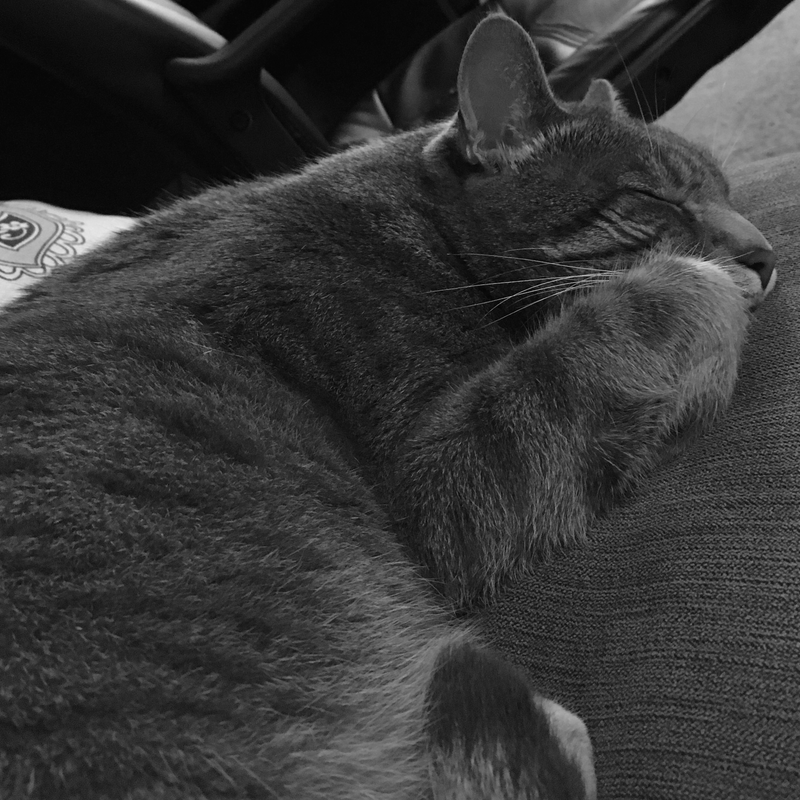
\includegraphics[width=0.5\textwidth]{chap4/figures/charles_gray.png}
	
\includegraphics[width=0.5\textwidth]{chap4/figures/charles_block.png}
	\caption{{\em{\bf Left:} The original $800 \times 800$ image.} {\em{\bf Right:} An $8 \times 8$ sub-block zoomed in.}}
	\label{fig:charles}
\end{figure}

\begin{equation}
	\BB = \begin{pmatrix}
	56 & 42 &	46 &	43 &	46 & 48 &	43 &	48\\
	45 &	47 &	59 & 	47 &	57 &	50 &	50 &	65\\
	48 &	59 &	37 &	41 &	45 &	52 &	67 &	74\\
	51 &	39 &	47 &	50 &	55 &	70 &	54 &	36\\
	39 &	66 &	59 &	72 &	88 &	49 &	26 &	20\\
	66 &	69 &	76 &	75 &	50 &	24 &	25 &	25\\
	70 &	78 &	79 &	38 &	20 &	23 &	22 &	20\\
	75 &	56 &	27 &	23 &	23 &	23 &	26 &	56
	\end{pmatrix}
	
\label{eq:subblock}
\end{equation}

To exploit the redundancy of the image in the frequency domain, we now transform each block according to a two-dimensional discrete cosine transform (2D-DCT). The discrete cosine transform, with some massaging, can actually be regarded as a particular case of the discrete Fourier transform, so conceptually, we can regard it in the same spirit. The resulting data transforms $\BB$ into $\textnormal{DCT}\left(\BB\right) = \widehat{\BB}$ as follows:

\begin{equation}
	\widehat{\BB} = \begin{pmatrix}
	388.13   &   48.51   &   3.43   &   -5.62   &   3.63   &   -10.51   &   1.42   &   2.12\\
	21.90     &	 -65.26   & -10.63  &  10.88   &   -0.39  &	1.66     & 	2.68	  &   2.75\\
	-27.13    &   5.92     &   53.83 &   -8.29   &	 5.35   &	1.02	    & 11.21   &   0.80\\
	6.26	      &   45.24   & -45.46  & -13.37  &	 1.97   &	3.12     &	0.07    &   6.32\\
	-12.63    &	-15.30    & -11.94  &	28.36   &	11.38  &	-4.05    & 1.56	   &  -3.43\\
	-8.00	      &   9.89     &   14.93  &  5.72     &	-20.23 &   16.34   &  9.22     &   -2.35\\
	0.82	      &   -8.88    &   17.96  &	-0.44    &  13.89   &    4.13	    & -10.33   & -7.66\\
	0.16	      &   3.34     &   -1.24   & 	-2.58    & 	-5.01	   &   -15.33  & -11.65   &  -0.71	
	\end{pmatrix}
\label{eq:dct2}
\end{equation}

\begin{figure}
\label{fig:jpeg8}
	\centering
	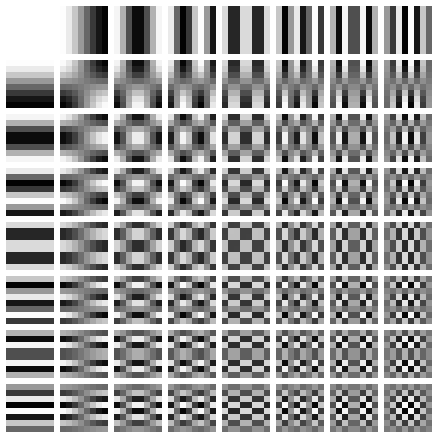
\includegraphics[width=0.5\textwidth]{chap4/figures/jpeg8.png}
	\caption{\em The $64$ 2D-DCT basis vectors for an $8 \times 8$ domain. Any $8 \times 8$ image can be expressed as a linear combination of these vectors. For example, the $8 \times 8$ array in \ref{eq:dct2} gives the corresponding weights that would generate the original sub-block $\BB$ in \ref{eq:subblock}.}
\end{figure}

Next, we {\em dampen} the frequencies by point-wise dividing the resulting set of values by a pre-determined damping array, $\QQ$, given by Equation \ref{eq:q50}. 
\begin{equation}
	\QQ = \begin{pmatrix}
	16 & 11 & 10 & 16 & 24 & 40 & 51 & 61\\
	12 & 12 & 14 & 19 & 26 & 58 & 60 & 55\\
	14 & 13 & 16 & 24 & 40 & 57 & 69 & 56\\
	14 & 17 & 22 & 29 & 51 & 87 & 80 & 62\\
	18 & 22 & 37 & 56 & 68 & 109 & 103 & 77\\
	24 & 35 & 55 & 64 & 81 & 104 & 113 & 92\\
	49 & 64 & 78 & 87 & 103 & 121 & 120 & 101\\
	72 & 92 & 95 & 98 & 112 & 100 & 103 & 99	
	\end{pmatrix}
\label{eq:q50}	
\end{equation}

The goal of this procedure is to dampen enough of the frequencies to values small enough that, upon integer rounding, they become zero. This allows for compression gains, albeit at the cost of information loss. Equation \ref{eq:round} shows the result.

\begin{equation}
	\textnormal{Round}\left(\frac{\widehat{\BB}}{\QQ}\right) = \begin{pmatrix}
	24 &	4 &	0 &	0 &	0 &	0 &	0 &	0\\
	2 &	-5 &	-1 &	1 &	0 &	0 &	0 &	0\\
	-2 &	0 &	3 &	0 &	0 &	0 &	0 &	0\\
	0 &	3 &	-2 &	0 &	0 &	0 &	0 &	0\\
	-1 &	-1 &	0 &	1 &	0 &	0 &	0 &	0\\
	0 &	0 &	0 &	0 &	0 &	0 &	0 &	0\\
	0 &	0 &	0 &	0 &	0 &	0 &	0 &	0\\
	0 &	0 &	0 &	0 &	0 &	0 &	0 &	0
	\end{pmatrix}
\label{eq:round}
\end{equation}

Note how many of the entires have been dampened to zero, as desired. Next, we scan through this array in a zigzag fashion, as demonstrated by Figure \ref{fig:zigzag}.

\begin{figure}
	\centering
	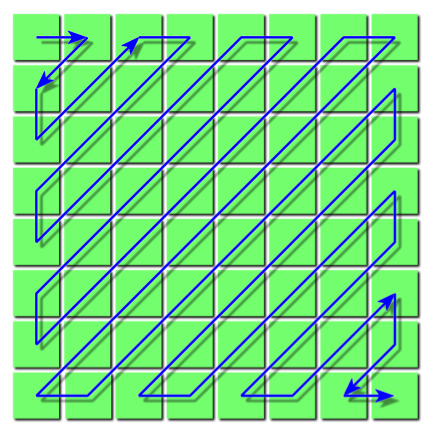
\includegraphics[width=0.5\textwidth]{chap4/figures/zigzag.png}
	\caption{\em The zigzag scan from northwest to southeast corner. The goal is to catch long consecutive strings of zeroes.}
	\label{fig:zigzag}
\end{figure}

This allows us to catch long strings of zeroes. In this case, the final $31$ entries are all zeroes, so run-length coding will prove to be highly profitable. Although the full JPEG standard includes several additional wrinkles, these are beyond the scope of the current discussion.

The decoding procedure is a straightforward reversal of each of the coding steps: for each block, we first decode the run-length code, we unzigzag the data into the correct shape, we undampen it by multiplying by $\QQ$, and finally, we compute the inverse two-dimensional discrete cosine transform (inverse 2D DCT). Figure \ref{fig:blockrecon} shows the JPEG-decoded block side-by-side with its original counterpart. The overall average error in this block comes out to approximately $7$ values per pixel (on a $256$-value grayscale). Figure \ref{fig:comp_comparison} shows the whole image compressed. The average error across the whole image comes out to about $4$ values per pixel, with an overall compression ratio of around $8 : 1$. Despite artifacts being noticeable at the block level when zoomed in, as in Figure \ref{fig:blockrecon}, the overall image has no visible artifacts. 

Lossy compression typically has a `sweet spot'---that is, a level of compression that achieves a significant data reduction without introducing noticeable artifacts. We also see in Figure \ref{fig:comp_comparison} the effect of going beyond this sweet spot and destroying the image quality: here, despite the attractive $100 : 1$ compression ratio, the image is unacceptably distorted.

\begin{figure}

	\centering
	
\includegraphics[scale=20]{chap4/figures/charles_block.png}
	
\includegraphics[scale=20]{chap4/figures/charles_block_reconstructed.png}
	\caption{{\em{\bf Left:} The original, uncompressed $8\times8$ data block.} {\em{\bf Right:} The same $8 \times 8$ block after undergoing JPEG compression at quality $50$ percent. Observe the general smoothing, which is an artifact of the information lost during the dampening and rounding stage.}}
\label{fig:blockrecon}
\end{figure}

\begin{figure}[H]
	\centering
	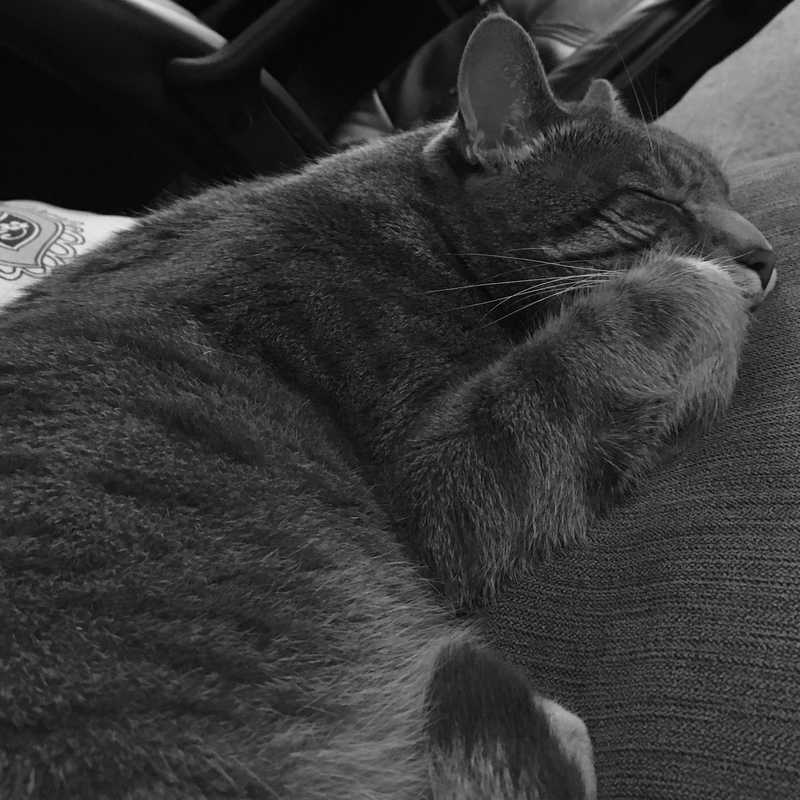
\includegraphics[width=0.4\textwidth]{chap4/figures/charles_gray_50.jpg}
	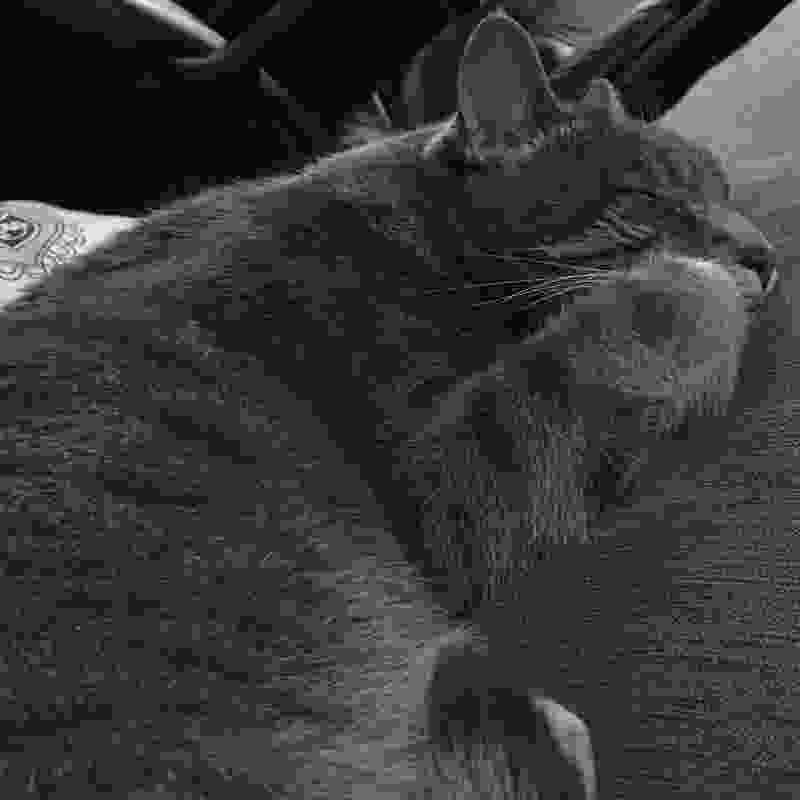
\includegraphics[width=0.4\textwidth]{chap4/figures/charles_gray_5.jpg}
	\caption{{\em{\bf Left:} A compression ratio of $8 : 1$ is achieved using the $50$ percent quality damping array with no visible artifacts.} {\em{\bf Right:} A compression ratio of $100 : 1$ is achieved using the $5$ percent quality damping array; however, there are many visible artifacts.}}
\label{fig:comp_comparison}
\end{figure}

\section{A Subspace Compression Scheme}
\label{sec:Algorithm}

\subsection{Compression Basis Selection}
\label{sec:laplacian}

In order to design a compression scheme for the velocity fields that comprise the columns of $\UU$, we must first select a transform basis that would ideally result in extremely sparse fields. Both discrete cosine transform (DCT) \cite{Yeo:1995:VRD} and wavelet \cite{guthe2002,treib12turbulence} bases have been successfully used in the past to compress scalar volumes, so they are promising candidates for velocity fields. We choose to use DCT because we observe that in the special case of Laplacian Eigenfunctions \cite{DeWitt:2012}, they actually yield ideal compression. The eigenfunctions inside a closed 3D box take the general form:
\begin{equation}
\begin{split}
\uu_x(k_1,k_2,k_3) &= \kappa_x \sin(k_1 x) \cos(k_2 y) \cos(k_3 z) \\
\uu_y(k_1,k_2,k_3) &= \kappa_y \cos(k_1 x) \sin(k_2 y) \cos(k_3 z) \\
\uu_z(k_1,k_2,k_3) &= \kappa_z \cos(k_1 x) \cos(k_2 y) \sin(k_3 z),
\end{split}
\end{equation}
where $\uu_x, \uu_y,$ and $\uu_z$ respectively represent the $x$, $y$, and $z$ components of a velocity field. The $k_i$ coefficients determine the frequency content of the field, and the three $\kappa$ terms are scaling coefficients that are derived from $k_i$.

\begin{figure}
\label{fig:laplacians}
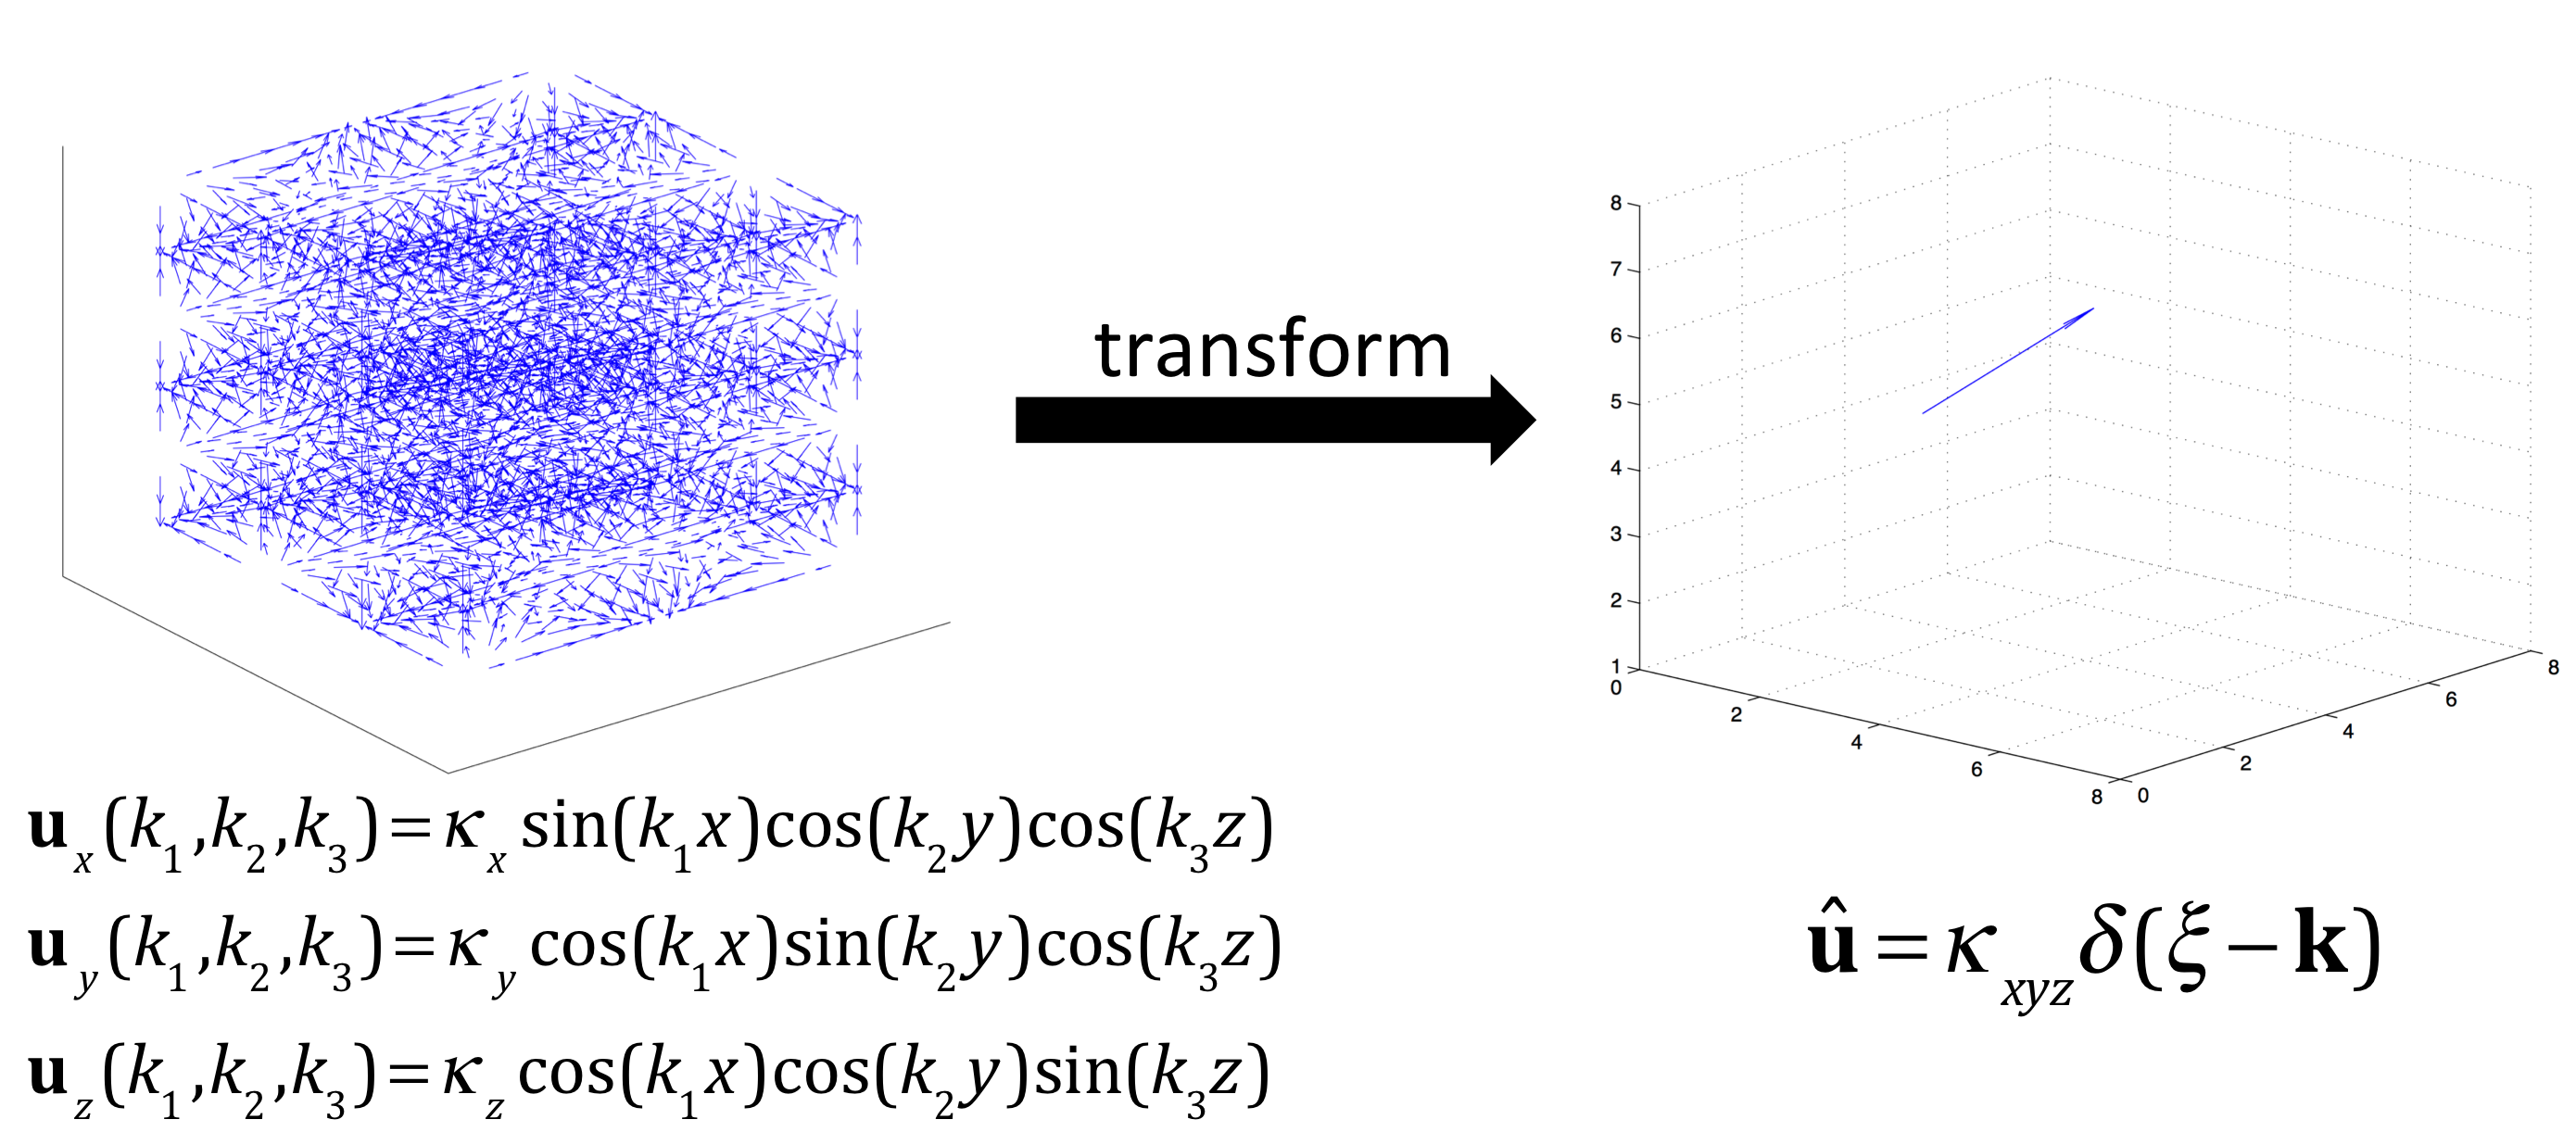
\includegraphics[width=\textwidth]{chap4/figures/laplacian_sparsity.png}
\caption{\em An eigenfunction of the Laplacian operator transforming into a delta function in frequency space.}
\end{figure}

We make the straightforward observation that the spatially varying components of each of these functions are purely trigonometric functions, so by applying appropriately interleaved DCTs and discrete sine transforms (DSTs) to these fields, they can be reduced to delta functions, regardless of their spatial frequency. In the notation of Long and Reinhard \cite{long2009}, if we use $\fancyF_\textrm{SCC}$ to denote a DST in the $x$ direction and DCTs in the $y$ and $z$ directions, we obtain,
\begin{equation}
\fancyF_\textrm{SCC}\left[\kappa_x\sin(k_1 x) \cos(k_2 y) \cos(k_3 z)\right] = \kappa_x\delta(k_1, k_2, k_3),
\end{equation}
where $\delta(k_1, k_2, k_3)$ is a delta function in SCC frequency space located at the $(k_1, k_2, k_3)$ grid cell. Similar transforms, e.g.~$\fancyF_\textrm{CSC}$ and $\fancyF_\textrm{CCS}$ can be used to generate delta functions for $\uu_y$ and $\uu_z$. Thus, any eigenfunction can be compressed down to three integers (the $k_i$s) and three floats (the $\kappa$ terms).

Asymptotically, this mixed DCT/DST losslessly transforms an $O(N)$ eigenfunction down to $O(1)$; no sparser representation is possible. This result only applies to the ideal case of analytic divergence-free velocity fields defined on the interior of a box. However, the high compression it achieves is encouraging, and motivates our further use of DCT to compress more general divergence-free fields.

\subsection{DCT-Based Compression}

Following from the previous discussion, we design a DCT-based, JPEG-like compression scheme. Each column of $\UU$ represents a vector field, and the columns are usually constructed using an SVD. Since this SVD has already minimized the amount of redundant information between columns, we compress them separately. Each column contain $x$, $y$ and $z$ velocity components, and we extract each of these components and compress them separately. Thus, if we describe the encoding procedure for a single scalar field, it can be applied to each velocity component of each column of $\UU$.

Analogously to JPEG, given a 3D scalar field, we decompose it into small blocks of size $b \times b \times b$, adding continuous extra padding in the case that one or more resolutions are not evenly divisible by $b$. We then perform a 3D-DCT on each block. In anticipation of quantization, the result is then normalized so that the largest frequency-domain value maps to the largest signed value for a 32-bit integer.

\noindent \textbf{Adaptive Quantization:} After transforming the signal to the frequency domain and normalizing the coefficients, as discussed in \S\ref{sec:jpeg}, the JPEG coding scheme then performs an element-wise division of the coefficients using a 2D quantization matrix in order to increase the likelihood that they will quantize to zero. In the JPEG standard, this matrix is adjusted depending on the quality setting; higher quality settings will have lower values to preserve more detail after dividing by the matrix, while lower quality settings will have higher values in the matrix to suppress more coefficients. For example, we previously saw in Equation \ref{eq:q50} the JPEG matrix corresponding to 50\% quality:

We index the matrix entries $\QQ(u,v)$ such that the upper-left corner, $\QQ(0,0) = 16$, corresponds to the DC component.  The entries of $\QQ$ were obtained from perceptual data \cite{Sayood:2012:JPEG}, and in general, higher frequency components have larger entries in order to suppress these coefficients which tend to carry less information than those in the lower frequencies.

Since we are not working with 2D color data but rather with 3D velocity fields, we need to construct a 3D version of this matrix, $\QQQ \in \R^{b \times b \times b}$. A close inspection of all of the complete matrix corresponding to Eqn.~\ref{eqn:quant} suggests that $\QQ(u,v) \propto u + v$, so a straightforward first attempt is:
\begin{equation}
\QQQ(u,v,w) = 1 + u + v + w.
\end{equation}
Other applications \cite{Yeo:1995:VRD} have used similar reasoning to arrive at similar matrices. However, while the 2D case has a suite of $\QQ$ matrices at its disposal that correspond to different levels of perceived visual quality, this data does not generalize to non-chromatic, 3D velocity data.

We instead propose to automatically generate a variety of different $\QQQ$ matrices during the compression stage. For each $b \times b \times b$ block, the energy is likely to reside in different frequencies, so we generate a custom matrix,
\begin{equation}
\QQQ(u,v,w) = (1 + u + v + w)^\gamma,
\end{equation}
where $\gamma$ is a parameter that is adjusted per block. Linear models are also possible, e.g.~$\QQQ(u,v,w) = \gamma\;(1 + u + v + w)$, but preliminary experiments found that this model was too simple to yield useful compressions. Analogous to the 2D case, the user specifies a quality parameter $p$. In 3D, we interpret $p$ as the percentage of the original energy\footnote{That is, $L_2$ norm.} that should be preserved. Each block then performs a bisection search over the range $\gamma \in [0, n]$, where $n = 32$ is the number of bits that were used for normalization prior to quantization. Higher values of $n$ are essentially meaningless, as they damp everything except the DC component to zero. In practice, we found that this bisection search terminates within a very small tolerance of the desired energy preservation after at most $8$ iterations.

This approach provides a custom quantization matrix for each block while maintaining an approximately constant energy loss per block. Important high-frequency components are preserved when they are present, while smoother, low-frequency blocks are still aggressively compressed. This block-varying value $\gamma$ must then be computed by the encoder and provided to the decoder in the encoded bytestream. For an $8 \times 8 \times 8$ block, the memory footprint of a single additional scalar $\gamma$ per block is negligible. We compare this strategy to a uniform non-adaptive quantization approach in \S\ref{sec:Results}.

\noindent \textbf{Flattening and Encoding:} After quantization, we convert the 3D array into a 1D array and perform run-length encoding \cite{Yeo:1995:VRD,Sayood:2012:JPEG}. No novel strategy needs to be devised for this component. The 3D to 1D conversion is performed in a zigzag pattern that is a straightforward 3D extension of the usual 2D JPEG ordering, which tries to group coefficients with similar sizes together in the bytestream.  In our case, the entries of $\QQQ(u,v,w)$ are arranged in increasing order of their sum $u + v + w$, which effectively clusters components with approximately the same frequency. The results are then run-length encoded in order to discover long runs of zeros.

\begin{figure}
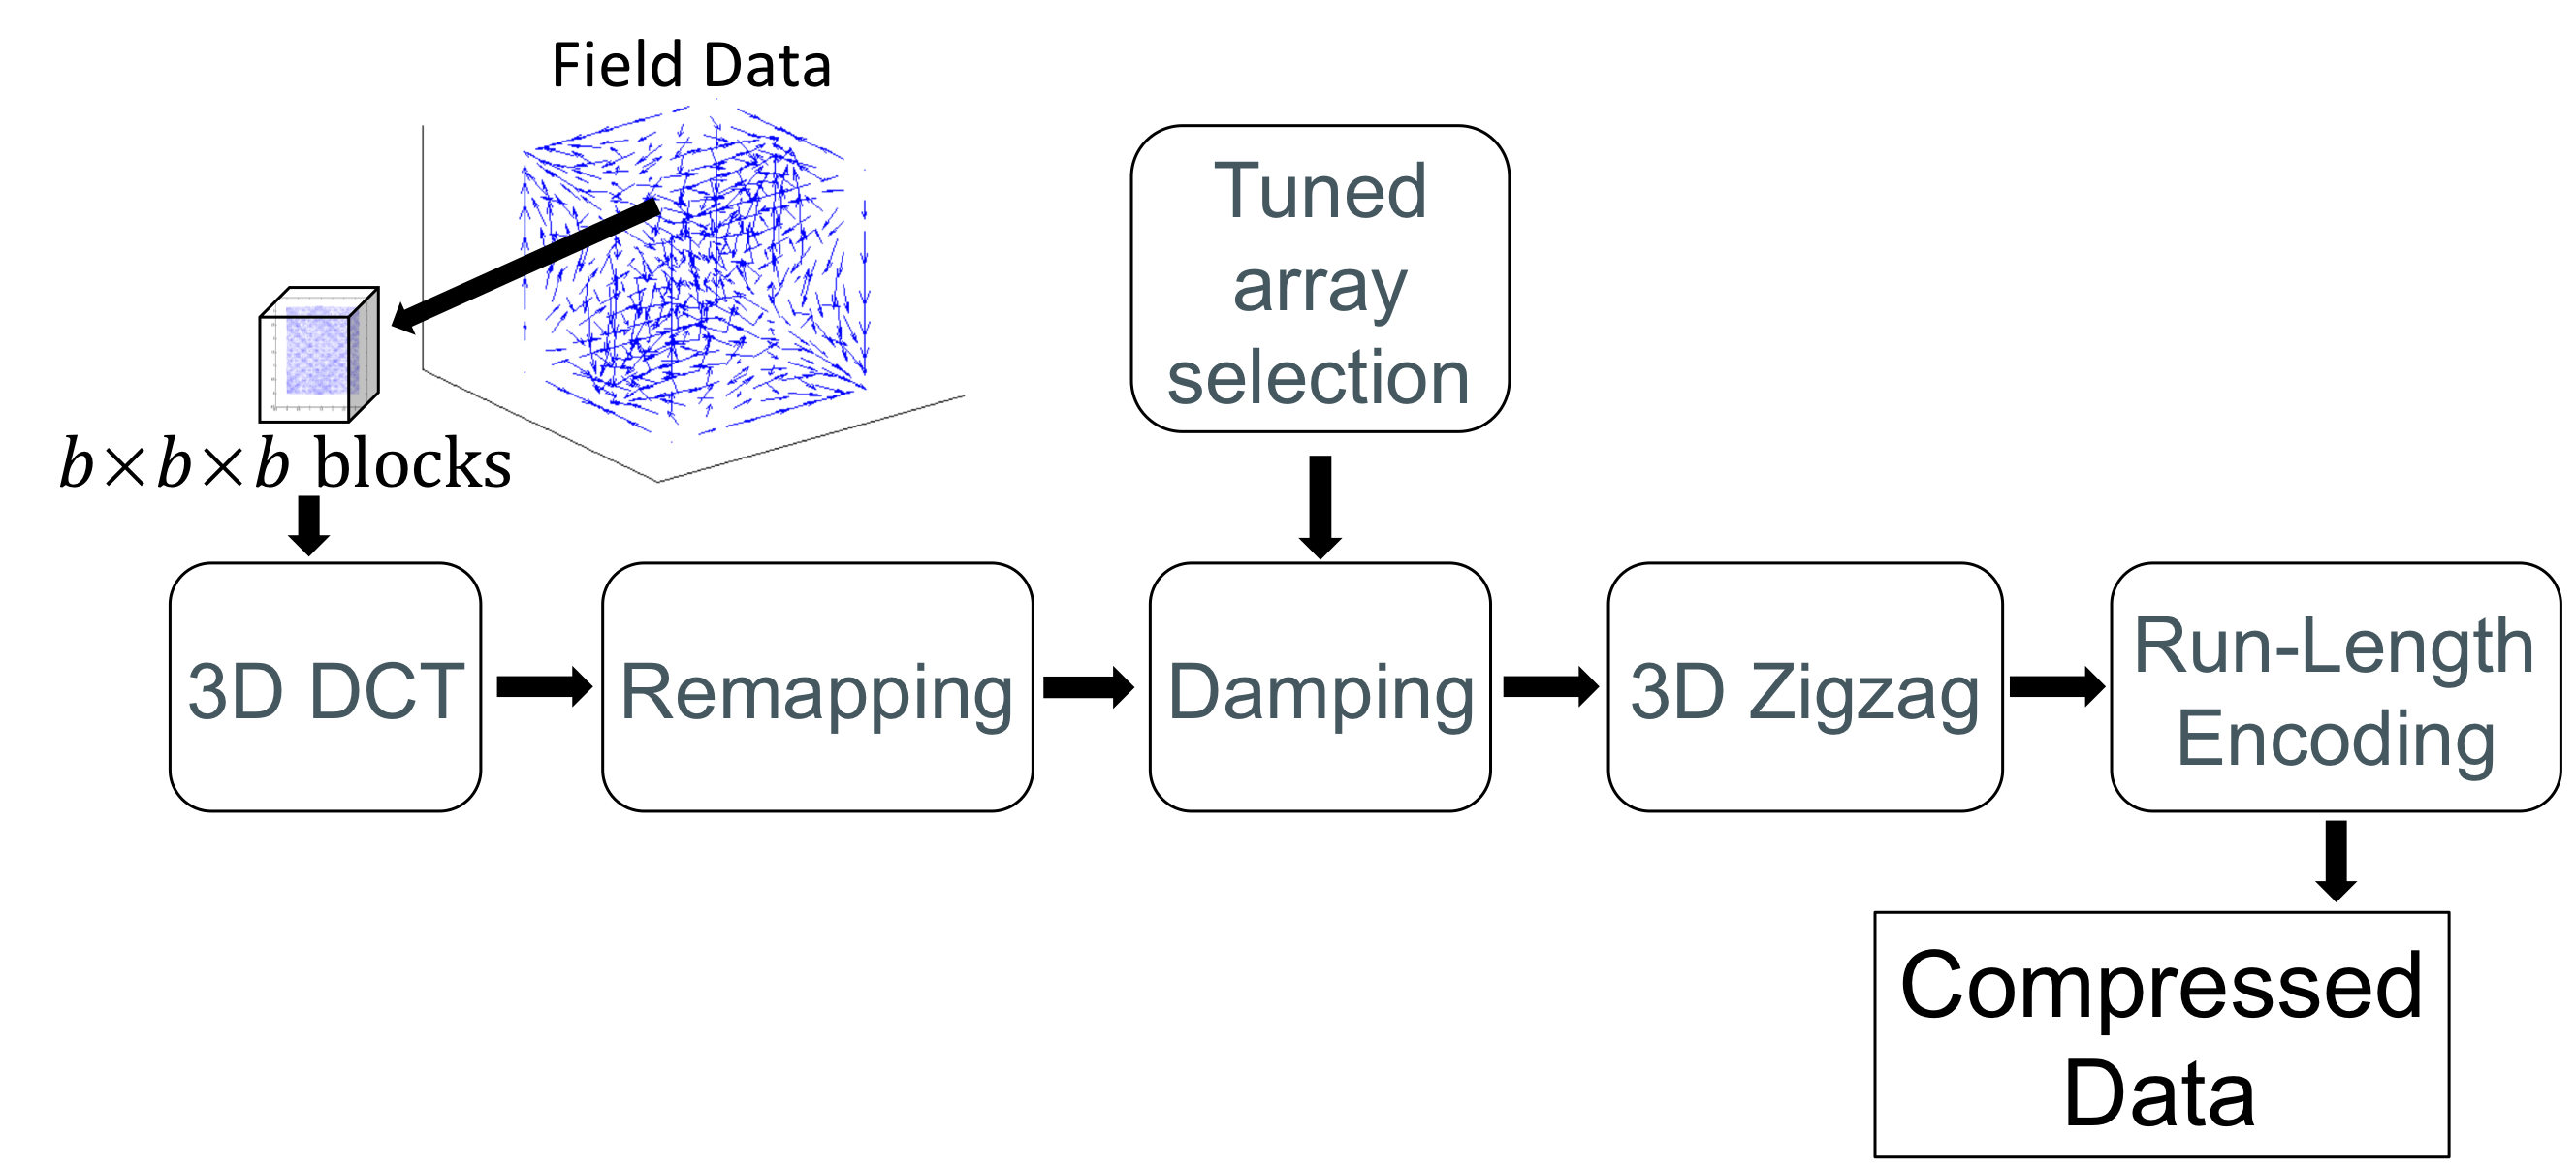
\includegraphics[width=\textwidth]{chap4/figures/compression_flowchart.png}
\caption{\em An overview of the encoding pipeline.}
\label{fig:flowchart}
\end{figure}

\begin{figure}
\centering
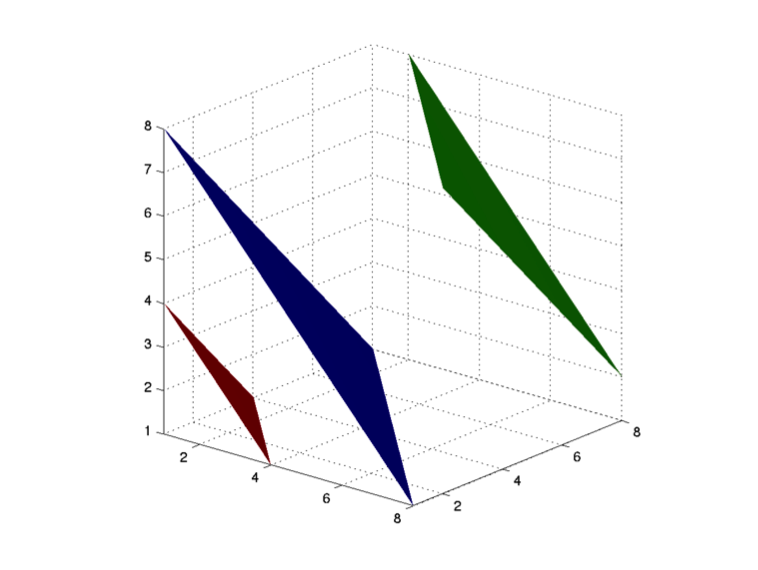
\includegraphics[width=0.5\textwidth]{chap4/figures/zigzag3d.png}
\caption{\em The 3D zigzag scan order. We move along slice planes of increasing index sum $c = 1 + u + v + w$.}
\label{fig:zigzag3d}
\end{figure}

\subsection{Subspace Decompression}
\label{sec:decompress}

\noindent \textbf{Batched Random Access:} The block-wise compression scheme we have described supports the batched random access requirements from \S\ref{sec:subspace} at runtime. For a single random access, the block containing the cell of interest is decompressed, which means the other $b \times b \times b - 1$ entries are potentially decoded needlessly. However, the coherency of the underlying incompressible flow tends to cluster cells of interest in the same blocks, so we did not find that this extra overhead created a major bottleneck.

The decompression proceeds in two stages, where an initial pass assembles the batch of requested cells and determines which blocks need to be decompressed. A second pass then decompresses the actual blocks. By consolidating the cell requests, it is guaranteed that no block is ever redundantly decompressed twice.

\noindent \textbf{Projection and Reconstruction:} The fast projection and reconstruction requirements from \S\ref{sec:subspace} are not as straightforward. A na\"{i}ve strategy is to decompress the entire matrix $\UU$ for each projection and reconstruction. For a given block size $B = b \times b \times b$, this results in $\frac{3N \times r}{B}$ DCTs and IDCTs at every timestep. These transforms dominate the running time (Table \ref{tab:naive-vs-sparse}), and largely negate the performance gains of the subspace approach. While memory savings are achieved, the speed-memory tradeoff is unacceptable.

However, we observe that both of the matrix-vector products $\UU\utilde = \uu$ and $\UU^T\uu = \utilde$ can be performed {\em sparsely in the frequency domain}. The projection operator then only performs a DCT on $\uu$, not all $r$ columns of $\UU$. This operation is permissible because the DCT is a unitary transform, and therefore preserves inner products. Specifically, if $\xx$ and $\yy$ are vectors in the spatial domain and $\xhat$ and $\yhat$ are their counterparts in the frequency domain, $\langle \xx, \yy \rangle = \langle \xhat, \yhat \rangle$, where $\langle \cdot, \cdot \rangle$ denotes the usual Euclidean inner product.

We define the following notation to describe the advantages of this approach. The frequency domain version of a quantity is denoted with a hat, e.g., $\UU$ with DCT applied to each column is $\Uhat$. The {\em lossy, compressed} version of $\Uhat$, where near-zero values have been quantized to zero, is denoted $\Chat$. The spatial domain version of $\Chat$ is correspondingly $\CC$. In essence, our compression scheme has introduced the approximations $\UU \approx \CC$ and $\Uhat \approx \Chat$.


Using the unitary property, we can see that if we use DCT to transform $\uu$ to $\uhat$, then $\UU^T\uu = \utilde$ is equivalent to $\Uhat^T\uhat = \utilde$. Using the compressed versions will yield a result slightly different from $\qq$, but the same relation holds: $\CC^T\uu = \Chat^T\uhat \approx \utilde$. The na\"{i}ve approach spends most of its time transforming $\Chat$ to $\CC$, but by constructing $\uhat$, we can avoid this stage altogether. Replacing the IDCT over all $r$ columns of $\Chat$ with a single DCT of $\uu$ is significant, because even for a modest $r = 10$, the number of transforms is reduced by an order of magnitude. Additionally, the $\Chat^T\uhat$ product can now exploit the sparsity of $\Chat$ that was discovered by the compression stage. Since $\Chat$ is static over the lifetime of a simulation, the location of all the zero entries can be cached, and these multiplies can be skipped. 

A fast reconstruction strategy then follows: $\Chat\utilde \approx \uhat$. The sparsity of $\Chat$ can again be exploited here, as each column $\Chat$ is scaled by an entry of $\utilde$, and all the multiplies with respect to zeroes can again be skipped. Once $\uhat$ is known, an IDCT can be performed on it once, and IDCTs over all $r$ columns of $\Chat$ is again avoided.

For a $\CC$ matrix containing ${3N \times r}$ non-zero entries, after taking the complexity of the DCTs and IDCTs into account, na\"{i}ve projection and reconstruction each take $O\left(3N \times r +\frac{3N \times r}{B} B \log B\right) = O\left((3N \times r)\log B\right)$ time. Using our approach, a $\Chat$ containing $S$ non-zero entries instead takes $O\left(S + \frac{3N}{B} B \log B\right) = O\left(S + 3N \log B\right)$ time. The $r$ factor has been removed as a multiplier of $\log B$, and replaced with the additive $S$ term. As seen in Table \ref{tab:naive-vs-sparse}, this results in speedups that approach an order of magnitude.

\subsection{Discussion}

We have described one possible scheme for compressing subspace fluid basis matrices. Several initially promising possibilities were also investigated, but ultimately discarded.

The motivating example from \S\ref{sec:laplacian} uses mixed DST and DCT to achieve ideal compression, whereas we only use DCT. The use of DST was investigated as well, but was not found to give superior results. Unless the velocity values along a block border are all exactly zero, i.e.~the block has Dirichlet boundaries along all its walls, the DCT consistently yields superior results.

The $\UU$ matrix is usually constructed using an SVD \cite{Treuille:2006:MRF,Kim2013} or an eigenanalysis \cite{DeWitt:2012,Liu:2015:MVF}. Therefore, corresponding singular values or eigenvalues are usually available for each column of $\UU$. These values could be used to guide the compressor, e.g.,~by allowing columns with unimportant singular values $\sigma_i$ to be compressed more aggressively. However, we found that the relationship between $\sigma_i$ and visual quality is not straightforward. Especially during re-simulation, columns that had unimportant $\sigma_i$ during the initial analysis can obtain large coefficients in $\utilde$. In such cases, the aggressive compression can become visible.

Prior to compression, an additional SVD could be run on each $b \times b \times b$ block in $\UU$ to determine if there is a superior coordinate system for compression other than the canonical $x$, $y$, and $z$ axes. However, the per-block rotation that this introduces breaks the fast matrix-vector multiply described in \S\ref{sec:decompress}. Thus, we put this aside in favor of the fast multiplies, but a method that supports both operations is an interesting direction for future work.


\begin{figure}
		\centering
		\includegraphics[height=0.5\textwidth]{chap4/figures/blockSpatial}
		\includegraphics[height=0.5\textwidth]{chap4/figures/blockFreq}
%		\vspace*{-1em}
		\caption{{\em{\bf Left:} An $8 \times 8 \times 8$ block of one of the velocity fields obtained from the Singular Value Decomposition.} {\em{\bf Right:} The same $8 \times 8 \times 8$ velocity field block in the frequency domain after taking a $3$D Discrete Cosine Transform. The sparsity not only allows for transform compression but also frequency-domain subspace projection speedups.}}
		\label{fig:sparseFreq}
\end{figure}













